\documentclass{standalone}

\usepackage{graphics}
\usepackage[dvipsnames,svgnames]{xcolor}

\usepackage{tikz,pgf,pgfplots,circuitikz}
\pgfplotsset{compat=1.15}
\usetikzlibrary{intersections,arrows.meta,angles,calc,3d,decorations.pathmorphing}
\usepackage[compat=1.1.0]{tikz-feynhand}

\usepackage{amssymb,amsfonts,amsthm,mathtools}
\usepackage{physics,braket,bm}

\begin{document}  
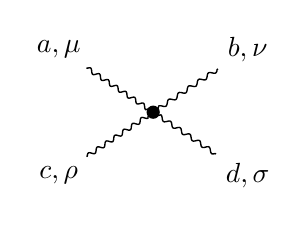
\begin{tikzpicture}[baseline=(o.base)]
  \begin{feynhand}
    \vertex[dot] (o) at (0,0){};
    \vertex[particle] (p1) at (-1.2,0.8) {$a,\mu$};
    \vertex[particle] (p2) at (1.2,0.8) {$b,\nu$};
    \vertex[particle] (p3) at (-1.2,-0.8) {$c,\rho$};
    \vertex[particle] (p4) at (1.2,-0.8) {$d,\sigma$};
    \propag[boson] (p1) to (o);
    \propag[boson] (p2) to (o);
    \propag[boson] (p3) to (o);
    \propag[boson] (p4) to (o);
  \end{feynhand}
\end{tikzpicture}
\end{document}
